\subsection{ORB-SLAM3}

ORB-SLAM3 is a KV-SLAM implementation which is popular in research contexts due to its performance, open source codebase, and usage of methods and techniques that are well-documented and widely understood. Figure \ref{fig:orb-slam3} shows a simplified diagram of the internal processes of ORB-SLAM3. ORB-SLAM3 supports a variety of input modalities including monocular and stereo cameras, RGBD cameras, and IMU data. The system splits work across multiple threads, allowing it to perform tracking, mapping, loop, closure, relocalization, and optimization concurrently. Trajectories are 

\begin{figure}[!ht]
    \centering
    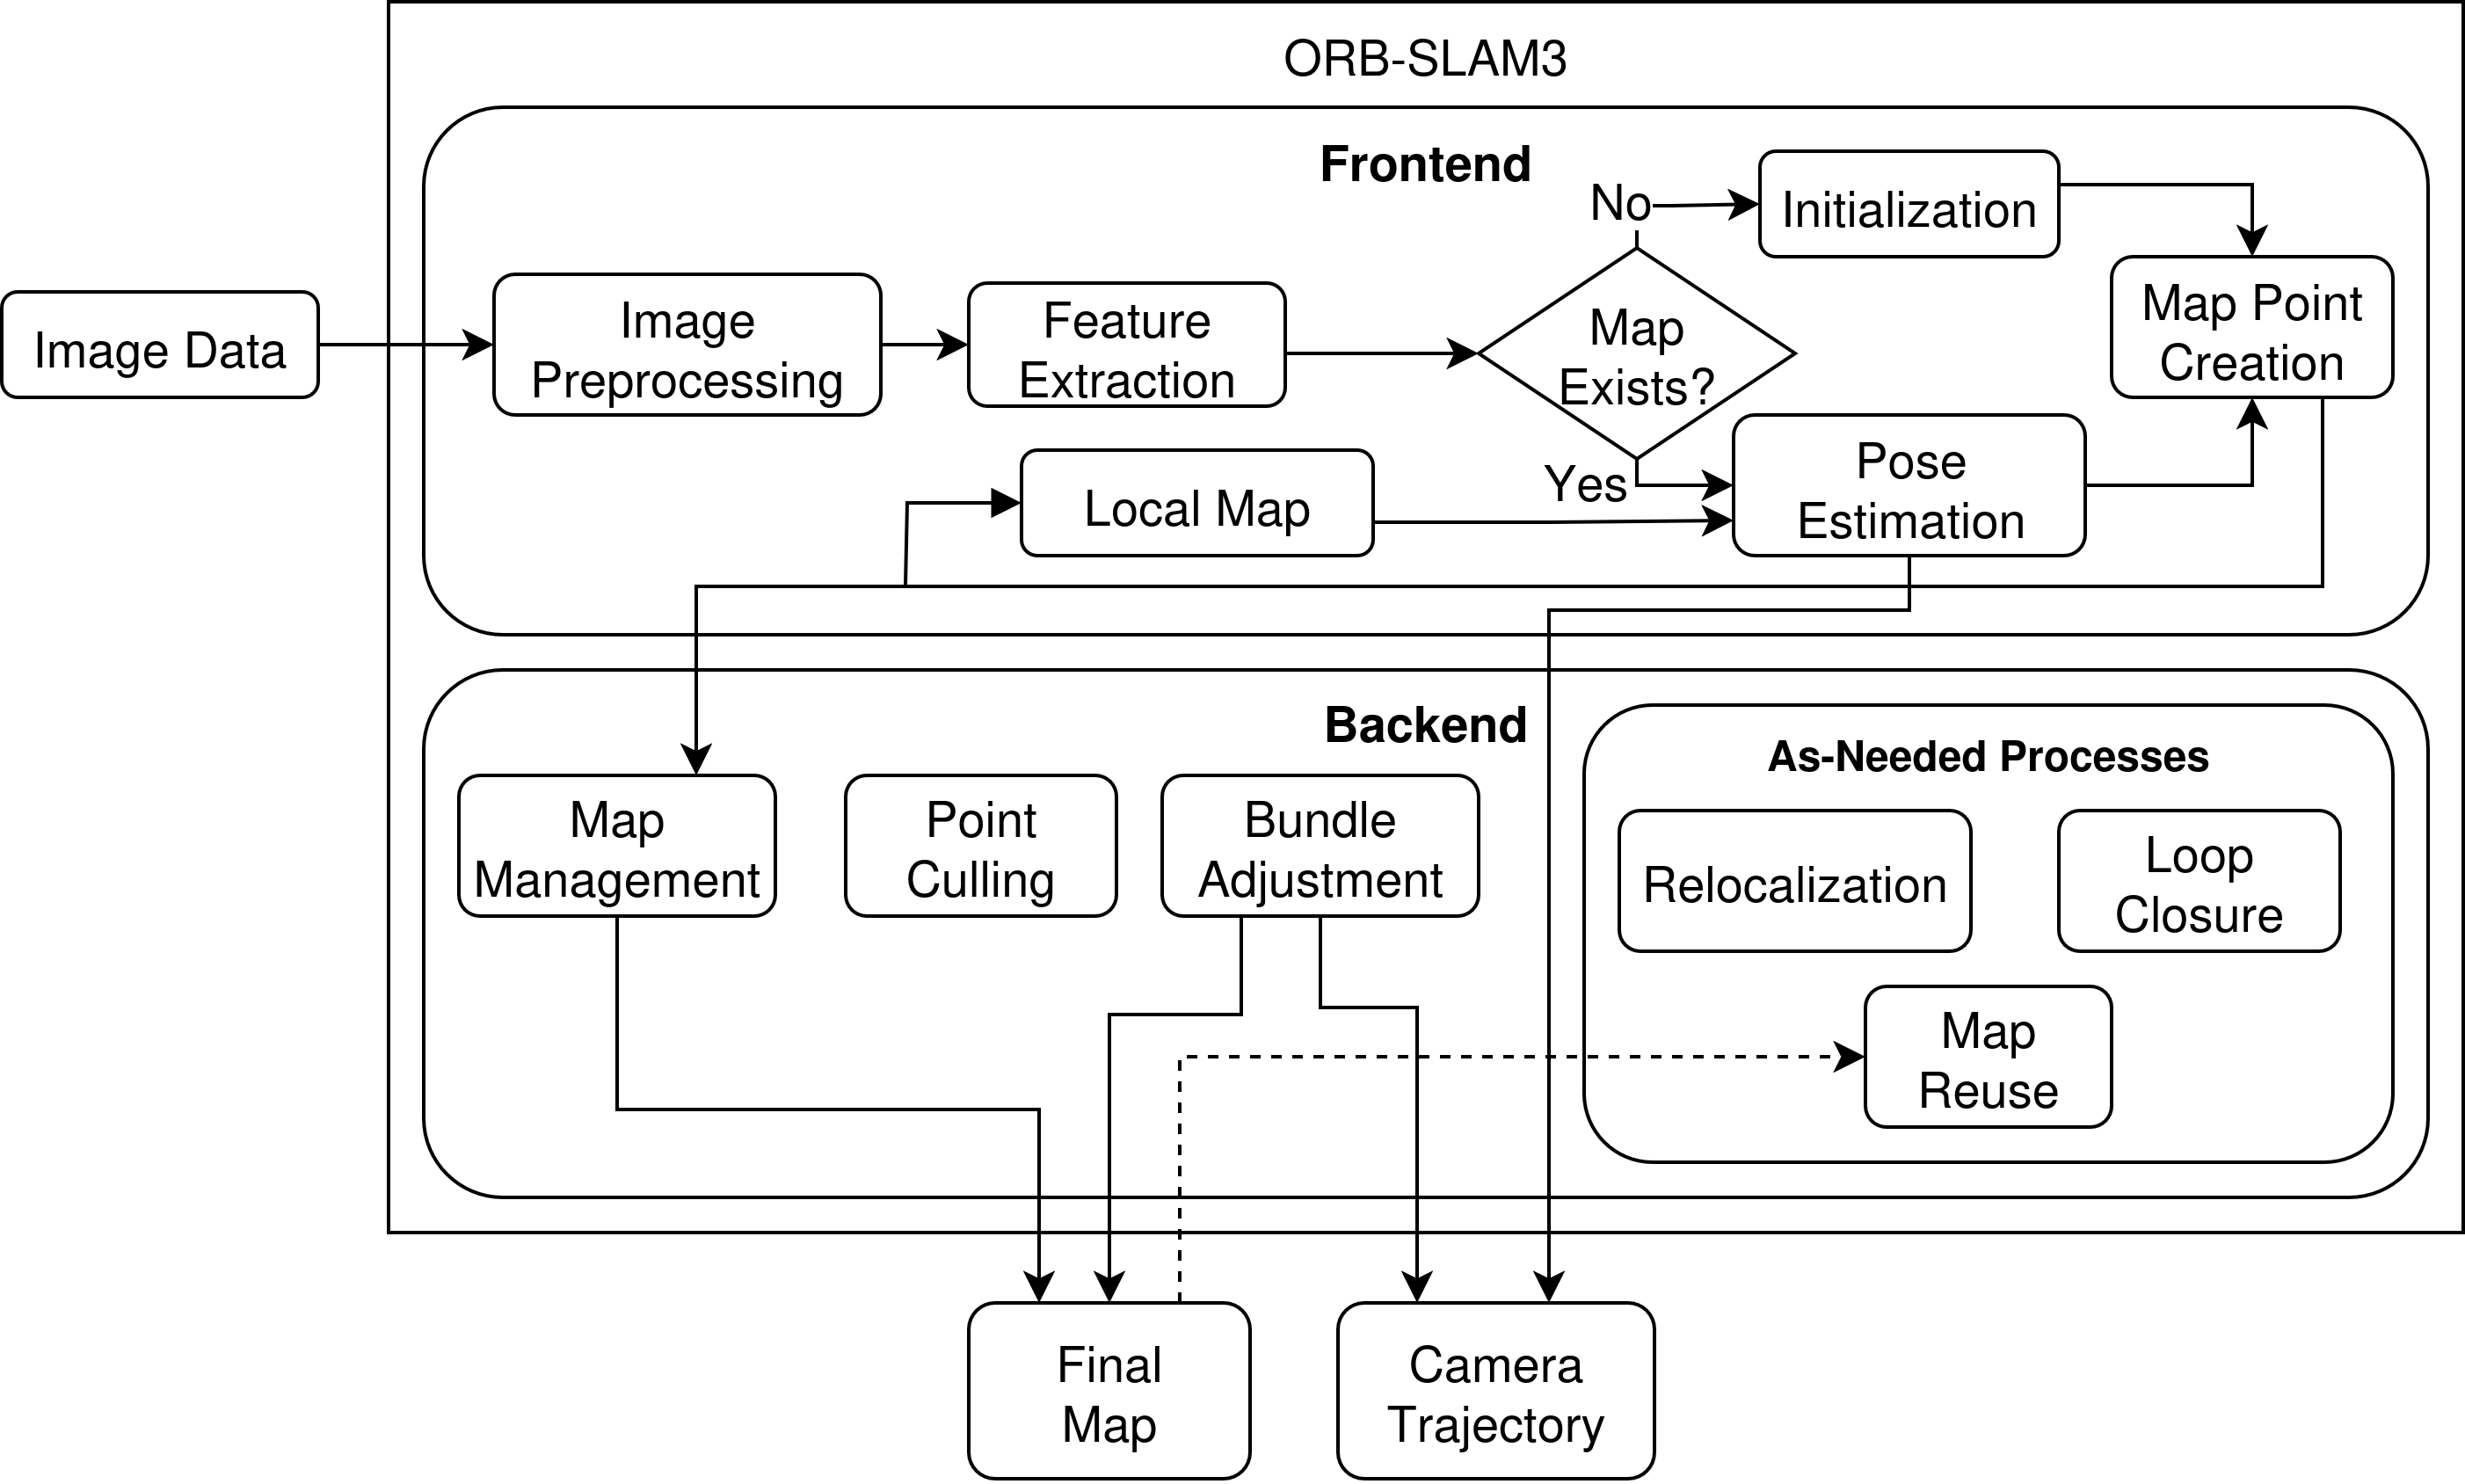
\includegraphics[width=0.9\textwidth]{resources/orb-slam3.png}
    \caption[Simplified ORB-SLAM3 Operational Diagram]{A simplified diagram of the inputs, outputs, and subprocesses of ORB-SLAM3.}
    \label{fig:orb-slam3}
\end{figure}